\documentclass[14pt]{extbook}
\usepackage{multicol, enumerate, enumitem, hyperref, color, soul, setspace, parskip, fancyhdr} %General Packages
\usepackage{amssymb, amsthm, amsmath, latexsym, units, mathtools} %Math Packages
\everymath{\displaystyle} %All math in Display Style
% Packages with additional options
\usepackage[headsep=0.5cm,headheight=12pt, left=1 in,right= 1 in,top= 1 in,bottom= 1 in]{geometry}
\usepackage[usenames,dvipsnames]{xcolor}
\usepackage{dashrule}  % Package to use the command below to create lines between items
\newcommand{\litem}[1]{\item#1\hspace*{-1cm}\rule{\textwidth}{0.4pt}}
\pagestyle{fancy}
\lhead{Makeup Progress Quiz 2}
\chead{}
\rhead{Version A}
\lfoot{5763-3522}
\cfoot{}
\rfoot{Spring 2021}
\begin{document}

\begin{enumerate}
\litem{
Construct the lowest-degree polynomial given the zeros below. Then, choose the intervals that contain the coefficients of the polynomial in the form $ax^3+bx^2+cx+d$.\[ \frac{4}{5}, \frac{3}{2}, \text{ and } \frac{7}{4} \]\begin{enumerate}[label=\Alph*.]
\item \( a \in [38, 45], b \in [-98, -95], c \in [-1, 4], \text{ and } d \in [76, 87] \)
\item \( a \in [38, 45], b \in [-167, -157], c \in [204, 222], \text{ and } d \in [-85, -78] \)
\item \( a \in [38, 45], b \in [22, 24], c \in [-118, -107], \text{ and } d \in [-85, -78] \)
\item \( a \in [38, 45], b \in [-167, -157], c \in [204, 222], \text{ and } d \in [76, 87] \)
\item \( a \in [38, 45], b \in [158, 163], c \in [204, 222], \text{ and } d \in [76, 87] \)

\end{enumerate} }
\litem{
Construct the lowest-degree polynomial given the zeros below. Then, choose the intervals that contain the coefficients of the polynomial in the form $x^3+bx^2+cx+d$.\[ -2 + 2 i \text{ and } 2 \]\begin{enumerate}[label=\Alph*.]
\item \( b \in [1.07, 2.48], c \in [-1.6, 0.7], \text{ and } d \in [-21, -13] \)
\item \( b \in [-3.13, -1.69], c \in [-1.6, 0.7], \text{ and } d \in [13, 22] \)
\item \( b \in [0.96, 1.95], c \in [-5.5, -3.4], \text{ and } d \in [4, 9] \)
\item \( b \in [0.96, 1.95], c \in [-1.6, 0.7], \text{ and } d \in [-9, -3] \)
\item \( \text{None of the above.} \)

\end{enumerate} }
\litem{
Which of the following equations \textit{could} be of the graph presented below?
\begin{center}
    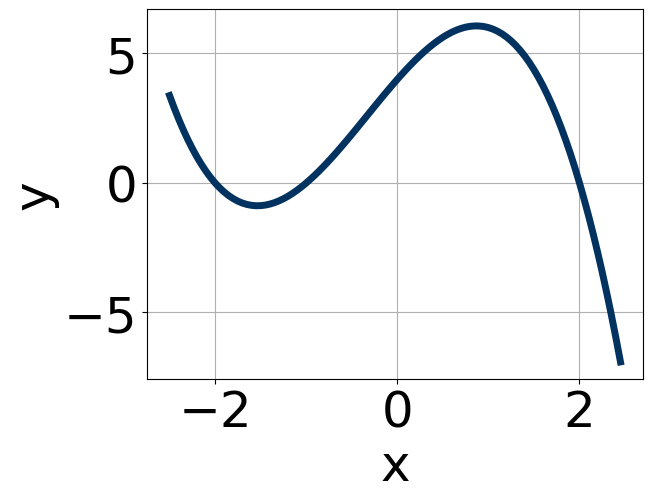
\includegraphics[width=0.5\textwidth]{../Figures/polyGraphToFunctionA.png}
\end{center}
\begin{enumerate}[label=\Alph*.]
\item \( 15(x + 1)^{9} (x - 2)^{5} (x + 2)^{7} \)
\item \( -14(x + 1)^{11} (x - 2)^{9} (x + 2)^{7} \)
\item \( 19(x + 1)^{6} (x - 2)^{5} (x + 2)^{9} \)
\item \( -13(x + 1)^{10} (x - 2)^{10} (x + 2)^{11} \)
\item \( -8(x + 1)^{10} (x - 2)^{7} (x + 2)^{9} \)

\end{enumerate} }
\litem{
Describe the zero behavior of the zero $x = 9$ of the polynomial below.\[ f(x) = -2(x + 9)^{2}(x - 9)^{7}(x - 4)^{5}(x + 4)^{9} \]\begin{enumerate}[label=\Alph*.]
\begin{multicols}{2}\item 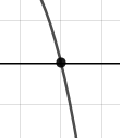
\includegraphics[width = 0.3\textwidth]{../Figures/polyZeroBehaviorCopyAA.png}\item 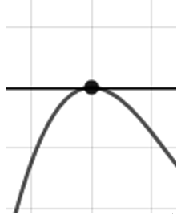
\includegraphics[width = 0.3\textwidth]{../Figures/polyZeroBehaviorCopyBA.png}\item 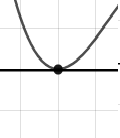
\includegraphics[width = 0.3\textwidth]{../Figures/polyZeroBehaviorCopyCA.png}\item 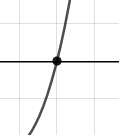
\includegraphics[width = 0.3\textwidth]{../Figures/polyZeroBehaviorCopyDA.png}\end{multicols}\item None of the above.
\end{enumerate} }
\litem{
Describe the zero behavior of the zero $x = 6$ of the polynomial below.\[ f(x) = -7(x + 2)^{4}(x - 2)^{2}(x + 6)^{5}(x - 6)^{4} \]\begin{enumerate}[label=\Alph*.]
\begin{multicols}{2}\item 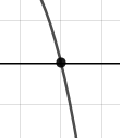
\includegraphics[width = 0.3\textwidth]{../Figures/polyZeroBehaviorAA.png}\item 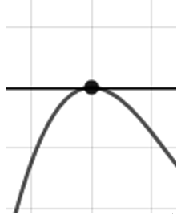
\includegraphics[width = 0.3\textwidth]{../Figures/polyZeroBehaviorBA.png}\item 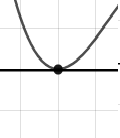
\includegraphics[width = 0.3\textwidth]{../Figures/polyZeroBehaviorCA.png}\item 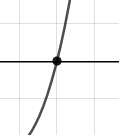
\includegraphics[width = 0.3\textwidth]{../Figures/polyZeroBehaviorDA.png}\end{multicols}\item None of the above.
\end{enumerate} }
\litem{
Construct the lowest-degree polynomial given the zeros below. Then, choose the intervals that contain the coefficients of the polynomial in the form $x^3+bx^2+cx+d$.\[ -5 - 2 i \text{ and } 2 \]\begin{enumerate}[label=\Alph*.]
\item \( b \in [-12, -4], c \in [4.8, 9.5], \text{ and } d \in [58, 60] \)
\item \( b \in [1, 4], c \in [-7.7, 1.2], \text{ and } d \in [-5, 3] \)
\item \( b \in [1, 4], c \in [2.7, 3.6], \text{ and } d \in [-11, -8] \)
\item \( b \in [3, 14], c \in [4.8, 9.5], \text{ and } d \in [-63, -54] \)
\item \( \text{None of the above.} \)

\end{enumerate} }
\litem{
Construct the lowest-degree polynomial given the zeros below. Then, choose the intervals that contain the coefficients of the polynomial in the form $ax^3+bx^2+cx+d$.\[ 4, \frac{7}{3}, \text{ and } \frac{1}{5} \]\begin{enumerate}[label=\Alph*.]
\item \( a \in [11, 20], b \in [13, 26], c \in [-145, -141], \text{ and } d \in [21, 36] \)
\item \( a \in [11, 20], b \in [98, 105], c \in [158, 162], \text{ and } d \in [21, 36] \)
\item \( a \in [11, 20], b \in [-101, -96], c \in [158, 162], \text{ and } d \in [21, 36] \)
\item \( a \in [11, 20], b \in [-101, -96], c \in [158, 162], \text{ and } d \in [-31, -27] \)
\item \( a \in [11, 20], b \in [89, 93], c \in [115, 123], \text{ and } d \in [-31, -27] \)

\end{enumerate} }
\litem{
Describe the end behavior of the polynomial below.\[ f(x) = -3(x + 2)^{5}(x - 2)^{6}(x + 6)^{4}(x - 6)^{6} \]\begin{enumerate}[label=\Alph*.]
\begin{multicols}{2}\item 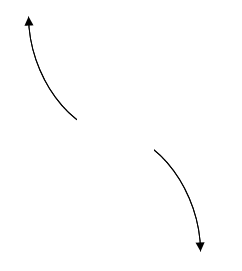
\includegraphics[width = 0.3\textwidth]{../Figures/polyEndBehaviorCopyAA.png}\item 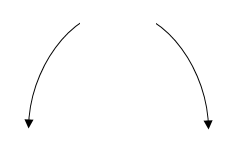
\includegraphics[width = 0.3\textwidth]{../Figures/polyEndBehaviorCopyBA.png}\item 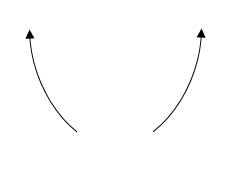
\includegraphics[width = 0.3\textwidth]{../Figures/polyEndBehaviorCopyCA.png}\item 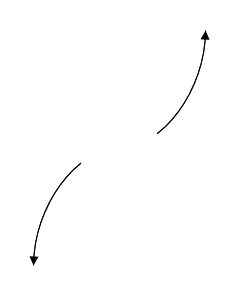
\includegraphics[width = 0.3\textwidth]{../Figures/polyEndBehaviorCopyDA.png}\end{multicols}\item None of the above.
\end{enumerate} }
\litem{
Which of the following equations \textit{could} be of the graph presented below?
\begin{center}
    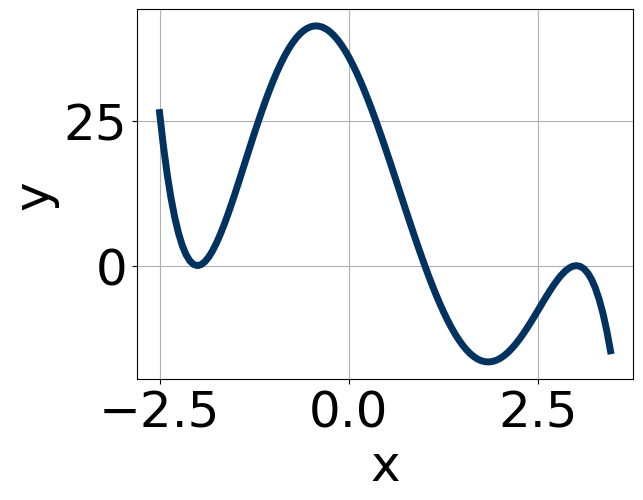
\includegraphics[width=0.5\textwidth]{../Figures/polyGraphToFunctionCopyA.png}
\end{center}
\begin{enumerate}[label=\Alph*.]
\item \( -5(x - 3)^{4} (x + 2)^{5} (x - 1)^{4} \)
\item \( -8(x - 3)^{10} (x + 2)^{5} (x - 1)^{9} \)
\item \( 4(x - 3)^{10} (x + 2)^{8} (x - 1)^{7} \)
\item \( -17(x - 3)^{8} (x + 2)^{4} (x - 1)^{11} \)
\item \( 20(x - 3)^{10} (x + 2)^{6} (x - 1)^{6} \)

\end{enumerate} }
\litem{
Describe the end behavior of the polynomial below.\[ f(x) = -8(x + 2)^{2}(x - 2)^{7}(x - 8)^{2}(x + 8)^{2} \]\begin{enumerate}[label=\Alph*.]
\begin{multicols}{2}\item 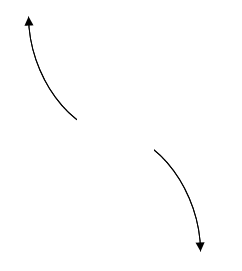
\includegraphics[width = 0.3\textwidth]{../Figures/polyEndBehaviorAA.png}\item 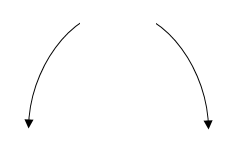
\includegraphics[width = 0.3\textwidth]{../Figures/polyEndBehaviorBA.png}\item 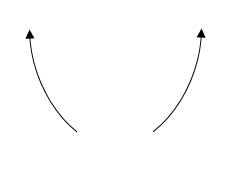
\includegraphics[width = 0.3\textwidth]{../Figures/polyEndBehaviorCA.png}\item 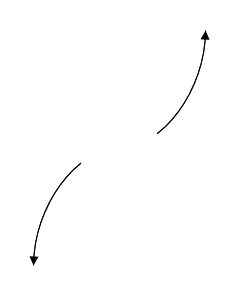
\includegraphics[width = 0.3\textwidth]{../Figures/polyEndBehaviorDA.png}\end{multicols}\item None of the above.
\end{enumerate} }
\end{enumerate}

\end{document}